\documentclass[12pt,preprint]{aastex}
%\documentclass{emulateapj}
\usepackage{amssymb,amsmath}
%\usepackage{caption}
%\DeclareCaptionLabelSeparator{dotemdash}{.--- }
%\captionsetup[figure]{labelformat=simple, labelsep=dotemdash}
%\usepackage{color,hyperref}
% hypertex insanity
%\definecolor{linkcolor}{rgb}{0,0,0.25}
%\hypersetup{
%  colorlinks=true,        % false: boxed links; true: colored links
%  linkcolor=linkcolor,    % color of internal links
%  citecolor=linkcolor,    % color of links to bibliography
%  filecolor=linkcolor,    % color of file links
%  urlcolor=linkcolor      % color of external links
%}
\newcounter{address}
\setcounter{address}{1}
%\usepackage{sidecap}
\setlength{\emergencystretch}{2em}%No overflowing references
\newcommand{\ie}{i.e.}
\newcommand{\etal}{et al.}
\newcommand{\dd}{\mathrm{d}}
\newcommand{\eg}{e.g.}
\newcommand{\eqnname}{equation}
\newcommand{\Eqnname}{Equation}
\newcommand{\equationname}{\eqnname}
\renewcommand{\tablename}{Table}
\renewcommand{\figurename}{Figure}
\newcommand{\figurenames}{\figurename~s}
\newcommand{\sectionname}{$\mathsection$}
\newcommand{\normal}{\ensuremath{\mathcal{N}}}
\newcommand{\flag}[1]{\texttt{\lowercase{#1}}}
\newcommand{\feh}{\ensuremath{[\mathrm{Fe/H}]}}
\newcommand{\afe}{\ensuremath{[\alpha\mathrm{/Fe}]}}
\newcommand{\logg}{log g}
\newcommand{\Ro}{\ensuremath{R_0}}

\renewcommand{\vec}[1]{\ensuremath{\mathbf{#1}}}
\newcommand{\unitvec}[1]{\ensuremath{\mathbf{\hat{#1}}}}
\newcommand{\vecx}{\ensuremath{\vec{x}}}
\newcommand{\vecv}{\ensuremath{\vec{v}}}
\newcommand{\vech}{\ensuremath{\vec{H}}}
\newcommand{\vecj}{\ensuremath{\vec{J}}}
\newcommand{\vecp}{\ensuremath{\vec{p}}}
\newcommand{\vecn}{\ensuremath{\vec{n}}}
\newcommand{\veco}{\ensuremath{\vec{\Omega}}}
\newcommand{\veca}{\ensuremath{\boldsymbol\theta}}
\newcommand{\df}{\ensuremath{f}}
\newcommand{\tdf}{\ensuremath{\mathrm{tDF}}}
\newcommand{\paramsdiff}{\ensuremath{\vec{p}_\Delta}}
\newcommand{\paramsdf}{\ensuremath{\vec{p}_{\mathrm{DF}}}}
\newcommand{\paramspot}{\ensuremath{\vec{p}_\Phi}}

\newcommand{\DF}{\df}
\newcommand{\dff}{\ensuremath{\mathbf{f}}}
\newcommand{\dex}{\ensuremath{\,\mathrm{dex}}}
\newcommand{\Myr}{\ensuremath{\,\mathrm{Myr}}}
\newcommand{\Gyr}{\ensuremath{\,\mathrm{Gyr}}}
\newcommand{\kpc}{\ensuremath{\,\mathrm{kpc}}}
\newcommand{\pc}{\ensuremath{\,\mathrm{pc}}}
\newcommand{\kms}{\ensuremath{\,\mathrm{km\ s}^{-1}}}
\newcommand{\msun}{\ensuremath{\,\mathrm{M}_{\odot}}}
\newcommand{\inv}{\ensuremath{^{-1}}}

\newcommand{\jr}{\ensuremath{J_R}}
\newcommand{\jphi}{\ensuremath{J_\phi}}
\newcommand{\jz}{\ensuremath{J_Z}}
\newcommand{\lz}{\ensuremath{L_Z}}
\newcommand{\Or}{\ensuremath{\Omega_R}}
\newcommand{\Ophi}{\ensuremath{\Omega_\phi}}
\newcommand{\Oz}{\ensuremath{\Omega_Z}}
\newcommand{\ar}{\ensuremath{\theta_R}}
\newcommand{\aphi}{\ensuremath{\theta_\phi}}
\newcommand{\az}{\ensuremath{\theta_Z}}

%\submitted{}

\begin{document}

\title{Dynamical modeling of tidal streams}
\author{Jo~Bovy\altaffilmark{\ref{Hubble}}}
\affil{Institute for Advanced Study, Einstein Drive, Princeton, NJ 08540, USA}
\email{bovy@ias.edu}
\altaffiltext{\theaddress}{\label{Hubble}\stepcounter{address} Hubble fellow}

\begin{abstract} 
  I present a new framework for modeling the dynamics of cold tidal
  streams. The framework consists of simple models for the initial
  action--angle distribution of tidal debris as a function of time,
  which can be straightforwardly evolved forward in time. Taking
  advantage of the essentially one-dimensional nature of cold tidal
  streams, the transformation to position--velocity coordinates can be
  linearized and interpolated near a small number of points along the
  progenitor orbit, thus allowing for efficient computations of a
  stream's properties in observable quantities. I illustrate how to
  calculate the stream's track in different coordinate systems, how to
  quickly estimate the dispersion perpendicular to the track, and how
  to draw mock stream data. As a generative model, this framework
  allows one to compute the full probability distribution function and
  marginalize over or condition it on certain phase--space dimensions
  as well as convolve it with observational uncertainties. This will
  be instrumental in proper data analysis of stream data. In addition
  to providing a computationally-efficient practical tool for modeling
  the dynamics of tidal streams, the action--angle nature of the
  framework helps elucidate in exactly what manner streams do not
  follow single orbits, how the observed width of the stream relates
  to the velocity dispersion or mass of the progenitor, and how the
  progenitor of ``orphan'' streams could be located.

  The practical usefulness of the proposed framework crucially depends
  on the ability to calculate action--angle variables for any orbit in
  any gravitational potential. A novel method for calculating actions,
  frequencies, and angles in any static potential using a single orbit
  integration is described in an Appendix.
\end{abstract}

\keywords{
        dark matter
        ---
	Galaxy: halo
	---
        Galaxy: kinematics and dynamics
        ---
	Galaxy: structure
        ---
        galaxies: interactions
        ---
        stellar dynamics
}


\section{Introduction}

Tidal streams hold enormous promise as probes of both the large-scale
structure of the Milky Way (MW) halo's density distribution
\citep[\eg,][]{Johnston99a,Koposov10a} and its small-scale
fluctuations \citep{Carlberg09a,Carlberg12a}. However, two factors
have hampered the practical use of tidal streams in obtaining
constraints on the MW gravitational potential. First, streams do not
trace a single orbit, which has led to confusion over how to best fit
streams and over how problematic the single-orbit approximation really
is \citep{Eyre11a,Sanders13a}. Second, approaches that go beyond the
single-orbit assumption encounter practical difficulties of
computational cost and observational data quality making many of these
approaches impractical for real, noisy data
\citep{Sanders13b,PriceWhelan13a}. Observed gaps in tidal streams may
be due to interactions with dark--matter subhalos \citep{Yoon11a}, but
spurious underdensities could be created by the dynamics of stream
stars. This hinders our ability to use underdensities in star counts
along a tidal stream in order to constrain the number of encounters
with dark satellites and their masses \citep{Ngan14a}. Fast,
generative models of tidal streams would greatly benefit both of these
applications.

It has long been clear that the dynamics of tidal streams is most
simply described in terms of action--angle coordinates
\citep{Tremaine99a,Helmi99a}. Once a star has been tidally stripped
from the progenitor, the self-gravity of the stream can be neglected
and the orbital actions of a stream member are conserved while the
angles increase linearly with time. The action--angle structure of a
stream is therefore characterized by strong but straightforward
correlations between the actions and angles of stream members, the
exploitation of which is crucial for using streams to measure the host
gravitational potential \citep{Sanders13b}. The description of a
stream in action--angle coordinates also elucidates the connection
between the orbit and velocity dispersion (or mass) of the progenitor
and the action distribution of the tidal debris \citep{Eyre11a},
allowing simple physical models of the stream to be used and
constrained by observational data.

However, streams are observed in position--velocity coordinates and
for action--angle descriptions to be useful, we must be able to
calculate the transformation between these coordinate systems
efficiently. Until now this has required accurate phase--space data
\citep{Sanders13b} and specialized algorithms to calculate
action--angle coordinates that break down for the eccentric orbits on
which tidal-stream progenitors are typically found (that is, radial
and/or vertical actions of similar size as the angular momentum;
\citealt{Sanders12a}). However, even with Gaia, future stream data
will typically have large uncertainties compared to the intrinsic
dispersion of the stream and in particular the line-of-sight
velocities of the faintest stream members will not be observed for
many stars. Additionally, streams are superimposed on a non-negligible
background of field stars and background contamination cannot be
easily taken into account in any of the current stream-fitting
methods.

In this paper, I present a new method for modeling cold tidal streams
that fundamentally lives in frequency--angle space, because after
specifying the time at which a star was stripped, the stream
distribution function is essentially one-dimensional in this
space. While many of the results of this paper are more generally
valid, the fiducial stream model in this paper consists of a
three-dimensional (close to) Gaussian distribution of frequencies in
the stream, a three-dimensional Gaussian distribution of initial angle
offsets between stream members and the progenitor, and a uniform
distribution of stripping times; the frequency and angle distributions
are independent of stripping time. While this model oversimplifies the
real stripping process, it is argued that at least for constraining
the gravitational potential with stream data, this simple model is
likely unbiased. For detailed mock stream data, more elaborate models
of the stripping process as a function of time might be necessary and
I discuss how these could easily be incorporated into the proposed
framework.

To evaluate the model in position--velocity coordinates, the
transformation to and from action--angle coordinates is computed using
a novel method for calculating action--angle coordinates presented in
Appendix~\ref{sec:aa}. This transformation is linearized at a small
number of points along the progenitor orbit that span the width of the
stream. For cold streams, the separation between the stream track and
the progenitor orbit as well as the internal differences within the
stream are small, such that this linear approximation is accurate
enough. The linear approximation allows for fast evaluation of the
average stream location (the stream ``track'') in position--velocity
coordinates and efficient mock data generation. For a uniform
distribution of stripping times, an observed stream member's
phase--space probability distribution function (PDF) can be
analytically marginalized over stripping time, such that using the
linear approximation any evaluation---including marginalization and
uncertainty convolution---of the PDF is extremely rapid. This clears
the way for proper probabilistic inference of the Milky Way halo's
gravitational potential and progenitor properties using stream data
for individual stars.

This paper is outlined as follows. In \sectionname~\ref{sec:dynamics}
I briefly summarize the dynamics of tidal streams in terms of
action--angle coordinates. A generative model of a tidal stream in
frequency--angle coordinates is given in
\sectionname~\ref{sec:generative}. \sectionname~\ref{sec:track}
describes how to compute the stream's properties as a function of
angle along the stream, both in action--angle coordinates and in
poition--velocity coordinates. \sectionname~\ref{sec:mock} discusses
how to generate mock stream data using the generative model of a tidal
stream and in \sectionname~\ref{sec:pdf} I show how to calculate the
stream PDF for individual stream members as well as its
marginalization and convolution over missing and noisy directions. A
discussion and outlook is presented in
\sectionname~\ref{sec:discussion} and I conclude in
\sectionname~\ref{sec:conclusion}. In Appendix
\sectionname~\ref{sec:aa} a novel method for calculating actions,
frequencies, and angles for any orbit in any static gravitational
potential is presented.


%BOVY: reference point


\section{The dynamics of tidal streams}\label{sec:dynamics}

The dynamics of tidal streams both in real (position--velocity) and
action--angle space has been described by various previous authors
\citep[\eg,][]{Helmi99a,Tremaine99a,SomeJohnstonPaper,Sanders13b}. I
provide here a brief description of the dynamics of tidal streams that
is relevant for what follows.

In real space, a tidal stream forms as stars are stripped from a
progenitor some time $\Delta t$ in the past and then evolve (largely)
independently in a galaxy's host potential, moving away both in
position and velocity from the progenitor object as time goes
on. Thus, a star was offset by a small amount $(\Delta \vecx,\Delta
\vecv)$ from the position of the progenitor $(\vecx^p,\vecv^p)(-\Delta
t)$ at that time. Then the star orbited under the influence of the
same gravitational potential $\Phi$ as the progenitor until the
present day $(t=0)$, when it was observed: $(\vecx,\vecv)(t=0)$ =
$\vech_{\Delta t}(\vecx^p(-\Delta t)+\Delta \vecx,\vecv^p(-\Delta
t)+\Delta \vecv)$, where $\vech$ denotes the Hamiltonian flow from
$t=-\Delta t$ to $t=0$ (see \citealt{binneytremaine}); this is simply
the orbit of the star between these times. In phase-space this orbit
can be calculated by solving Hamilton's equations: $\dot{\vecx} =
\vecv; \dot{\vecv} = - \dd \Phi / \dd \vecx$.

In action--angle space the dynamics of stream formation is much
simpler. A star received an offset ($\Delta \vecj,\Delta \veca$) at
time $-\Delta t$ from the action--angle coordinates of the progenitor
$(\vecj^p,\veca^p)$, similar to the small offset ($\Delta \vecx,\Delta
\vecv)$ in the real--space description. The offset in the actions
corresponds to an offset in the frequencies $\Delta \veco$;
ultimately, this offset is responsible for the spreading of the stream
over long stretches on the sky. Because both the progenitor's angles and
the star's angles increase linearly with time, albeit at different
frequencies, the difference in the angles also increases linearly in
time. Therefore at time $t=0$ the difference in angles is
\begin{equation}
\Delta \veca(t=0) = \Delta \veca(-\Delta t) + \Delta \veco \Delta t\,,
\end{equation}
while the difference in actions is constant
\begin{equation}
\Delta \vecj(t=0) = \Delta \vecj(-\Delta t)\,.
\end{equation}
As the initial offset $\Delta \veca(-\Delta t$ in angles is small
compared to the growth $\Delta\veco\Delta t$, $\Delta \veca(t=0)
\approx \Delta \veco \Delta t$.

Thus, in action--angle coordinates, the dynamics of tidal-stream
formation is simplified to linear growth of small initial angle
differences due to small action/frequency differences. The angle
direction $\unitvec{\veco} \equiv \Delta \veco / | \Delta \veco|$
along which a star moves away from the progenitor is related to the
initial action offset by $\Delta \veco \approx (\partial^2 H
/ \partial \vecj \partial \vecj) \Delta \vecj$, in the limit of small
action offsets, as $\veco = \partial H / \partial \vecj$. For an
approximately one-dimensional stream to form, the Hessian matrix
$(\partial^2 H / \partial \vecj \partial \vecj)\large|_{\vecj^p}$ has
to be dominated by a single large eigenvalue; in this case the angle
difference of stars stripped from the stream at any time will fall
along approximately the same direction $\unitvec\veco$, and the stream
will essentially be one dimensional. In detail, because the
distribution of initial offsets $\Delta \vecj$ is not isotropic, the
direction $\unitvec \veco$ is not just determined by the potential
(through $H$) and the progenitor orbit, but also by the distribution
of $\Delta \vecj$, which is set through a combination of the internal
dynamics of the progenitor and the stripping process (see discussion
in \citealt{Sanders13b}). For dynamical modeling we can be agnostic
about the relative importance of all of these contributors to
$\unitvec \veco$ by flexible modeling of the distribution of $\Delta
\vecj$.


\section{Generative models of tidal streams}\label{sec:method}


The discussions of the dynamics of stream formation in the previous
section directly give rise of a generative model of a tidal stream. A
star in a tidal stream is \emph{generated} through being stripped a
time $\Delta t$ ago from a progenitor $(\vecx^p,\vecv^p) \equiv
(\vecj^p,\veca^p)$ by receiving a small offset $(\Delta \vecx,\Delta
\vecv) \equiv (\Delta \vecj,\Delta \veca)$. The offset then evolves
using the dynamical equations given in the previous section and the
star is observed at time $t=0$ (\ie, today). Because phase-space
density is conserved by Liousville's theorem, a probabilistic model
results by relating the likelihood $p(\vecx,\vecv|\vecp)$ (where
$\vecp$ denotes the set of all model parameters; see below) for the
observed phase-space position today to the distribution of initial
offsets. This probabilistic model can be marginalized over missing
observational data or extended to include a model for outliers.

\subsection{Real--space modeling}

In more detail, in the real--space approach the model can be specified
by: (a) the gravitational potential $\Phi$, (b) the current
phase-space position of the progenitor $(\vecx_p,\vecv_p)(t=0)$, which
can be integrated backwards in time by reversing the Hamiltonian flow
defined by $\Phi$, (c) the time $\Delta t_i$ at which each star was
removed from the progenitor, and (d) the distribution $f(\Delta
\vecx,\Delta \vecv|\paramsdiff)$, characterized by some parameters
$\paramsdiff$, of initial phase-space offsets from which the actual
offsets $(\Delta \vecx_i,\Delta \vecv_i)$ are drawn. In practice, $f$
can be taken to be a Gaussian, characterized by a width in position
$\sigma_x$ and in velocity $\sigma_v$, related to the tidal radius and
escape velocity of the progenitor, respectively. However, more
complicated models for the initial phase-space distribution of the
debris can be used here as well.

The probability for observing a star today at $(\vecx,\vecv)$ given
items (a) through (d) is then
\begin{align}\label{eq:realdft}
  p(\vecx_i,\vecv_i | \Phi,\vecx_p,\vecv_p,\Delta t_i,\paramsdiff) 
  & = p(\vecx_i(-\Delta t),\vecv_i(-\Delta t) | \Phi,\vecx_p,\vecv_p,\Delta t_i,\paramsdiff) \,,\nonumber\\
  & = p([\vecx_i-\vecx_p](-\Delta t),[\vecv_i-\vecv_p](-\Delta t) | \Phi,\vecx_p,\vecv_p,\Delta t_i,\paramsdiff) \,\nonumber\\
  & = p(\Delta\vecx_i(-\Delta t),\Delta\vecv_i(-\Delta t) | \Phi,\vecx_p,\vecv_p,\Delta t_i,\paramsdiff)\,,\\
  & = f(\Delta\vecx_i(-\Delta t),\Delta\vecv_i(-\Delta t) | \Phi,\vecx_p,\vecv_p,\Delta t_i,\paramsdiff)\, ,\nonumber
\end{align}
where the first equality holds because the Hamiltonian flow is unique
and conserves phase-space volume by Liousville's theorem and the
second one because the Jacobian of the transformation
$(\vecx_i,\vecv_i)(-\Delta t) \rightarrow (\vecx_i,\vecv_i)(-\Delta t)
- (\vecx_p,\vecv_p)(-\Delta t)$ is one. The final probability can be
evaluated using the parameters $\paramsdiff$ following (d).

The time $\Delta t_i$ at which a star was removed is unobservable and
the probability in \eqnname~(\ref{eq:realdft}) should therefore be
integrated over this time using a prior $p(\Delta t_i|\ldots)$, where
$\ldots$ indicates that this prior could depend on other factors such
as the potential and the progenitor orbit\footnote{For example, one
  could insist that stars are removed around pericenter
  passages.}. For simplicity, we can assume a uniform prior for the
times $\Delta t$. The probability for a single star then becomes
\begin{align}\label{eq:realdf}
  p(\vecx_i,\vecv_i | \Phi,\vecx_p,\vecv_p,\paramsdiff) & = \int \dd
  \Delta t_i \,p(\vecx_i,\vecv_i | \Phi,\vecx_p,\vecv_p,\Delta t_i,
  \paramsdiff)\,.
\end{align}
If the progenitor's current phase-space position is unknown, then this
probability should be further marginalized over $(\vecx_p,\vecv_p)$;
for multiple stars, this marginalization is done after multiplying the
individual-star likelihoods in \eqnname~(\ref{eq:realdf}).

In practice, the likelihood in \eqnname~(\ref{eq:realdf}) can be
calculated as follows: for a given potential $\Phi$ and progenitor
$(\vecx_p,\vecv_p)$, we (a) integrate the orbits of all stars
$(\vecx_i,\vecv_i)$ and (b) that of the progenitor backward in time for
many Gyr and record the phase-space positions over time on a grid $j$
in $\Delta^j_i$; (c) we evaluate $f(\Delta \vecx_i,\Delta
\vecv_i)(\Delta t^j_i)$ for all stars $i$ and times $j$; (d) $f(\Delta
\vecx_i,\Delta \vecv_i)(\Delta t^j_i)$ is then summed over $j$ and the
logarithm of that is summed over $i$. The most computationally
expensive part of this calculation is the integration of the various
orbits. The evaluation of the likelihood for different parameters
\paramsdiff\ of $f$ can be efficiently computed by caching the orbit
integrations of (a) and (b); different progenitor orbits
$(\vecx_p,\vecv_p)$ can also make use of the stored orbits in (a).

The approach outlined in this section is straightforward, but very
computationally expensive, as it requires large numbers of orbit
integrations to explore all plausible removal times $\Delta t$,
progenitor orbits, and potentials. Moreover, when the data have large
uncertainties, more orbit integrations are necessary to explore each
data points uncertainty range. While it might be possible to speed up
the computation through linear approximations for nearby orbits, the
action--angle formalism allows for significant and elegant
simplifications and I consider the real--space approach further.

\subsection{Action--angle stream modeling}

Similar as for the real--space approach, we can write down a
generative model for the positions and velocities ($\vecx_i,\vecv_i$)
of stars $i$ in a tidal stream in the action--angle formalism by
specifying: (a) the gravitational potential $\Phi$, (b) the current
action-angle coordinates of the progenitor $(\vecj_p,\veca_p)(t=0)$,
(c) the time $\Delta t_i$ at which each star was removed from the
progenitor, and (d) the distribution $f(\Delta \vecj,\Delta
\veca|\paramsdiff)$, characterized by some parameters $\paramsdiff$,
of initial phase-space offsets from which the actual offsets $(\Delta
\vecj_i,\Delta \veca_i)$ are drawn. In practice, $f$ can again be
taken to be a Gaussian, although more general models could take the
expected `bowtie' structure of the action distribution into account
(\citealt{Eyre11a}; see also \figurename~\ref{fig:gd1_jt}).

The probability for observing a star today at $(\vecx,\vecv)$ given
items (a) through (d) is then
\begin{align}\label{eq:aadft}
  p(\vecx_i,\vecv_i | \Phi,\vecj_p,\veca_p,\Delta t_i,\paramsdiff) 
  & = p(\vecj_i,\veca_i | \Phi,\vecj_p,\veca_p,\Delta t_i,\paramsdiff) \,,\nonumber\\
  & = p(\vecj_i-\vecj_p,\veca_i-\veca_p-\Delta \veco_i\Delta t_i | \Phi,\vecj_p,\veca_p,\Delta t_i,\paramsdiff) \,,\\
  & = f(\Delta \vecj_i,\Delta \veca_i(-\Delta t_i) | \Phi,\vecj_p,\veca_p,\Delta t_i,\paramsdiff) \,,\nonumber
\end{align}
where the first equality holds because the Jacobian of the
$(\vecx,\vecv)\rightarrow(\vecj,\veca)$ transformation is unity and
the second equality is a simple linear transformation. The final
probability can again be evaluated using the parameters
\paramsdiff\ following (d).

As in the real--space formalism, we should integrate
\eqnname~(\ref{eq:aadft}) over the time $\Delta t_i$ at which the star
is removed from the progenitor (cf.~\eqnname~[\ref{eq:realdf}]):
\begin{equation}\label{eq:aadf}
  p(\vecx_i,\vecv_i | \Phi,\vecj_p,\veca_p,\paramsdiff) = \int \dd
  \Delta t_i\, f(\Delta \vecj_i,\Delta \veca_i(-\Delta t_i) |
  \Phi,\vecj_p,\veca_p,\Delta t_i,\paramsdiff) \,.
\end{equation}
Without further assumptions the action-angle formalism proceeds in the
same way as the real--space formalism, evaluating
\eqnname~(\ref{eq:aadft}) for a grid $j$ of times $\Delta t_i^j$ and
summing $f(\Delta \vecj_i,\Delta \veca_i(-\Delta t^j_i) |
\Phi,\vecj_p,\veca_p,\Delta t_i,\paramsdiff)$ over $j$.

Even without further assumptions about the shape of $f(\Delta
\vecj,\Delta \veca|\paramsdiff)$, the action-angle formalism already
allows for a simplification over the real--space method. Because the
progenitor orbit is specified in action-angle coordinates, it can be
changed \emph{without} expensive orbit integrations of all possible
source orbits. As the progenitor's current phase-space position is a
six-dimensional parameter, this is a major simplification of the
dynamical model when the source orbit is unknown. Note that this
simplification does require us to be able to compute $\veco(\vecj)$,
to calculate the new source frequencies $\veco_p$ when changing the
source actions $\vecj_p$. This mapping can be constructed using a
small number of (action,frequency) calculations covering the range of
possible source actions and is relatively easy to construct due to the
approximately one-dimensional structure of a stream (see discussion at
the end of \sectionname~\ref{sec:dynamics}).

We can simplify \eqnname~(\ref{eq:aadf}) by assuming (a) that
$f(\Delta \vecj,\Delta \veca|\paramsdiff)$ is separable into
$f_{\veca}(\Delta \veca|\paramsdiff)\,f_{\vecj}(\Delta
\vecj|\paramsdiff)$ and (b) that the distribution $f_{\veca}(\Delta
\veca|\paramsdiff)$ is Gaussian. In what follows, we will assume that
this Gaussian is isotropic with dispersion $\sigma_\theta$, but all of
the results are the same after appropriate diagonalization and
rescaling of the angles for more general covariance matrices. In this
case, \eqnname~(\ref{eq:aadf}) can be written as
\begin{equation}
\begin{split}
  p(\vecx_i,\vecv_i & | \Phi,\vecj_p,\veca_p,\paramsdiff) 
   = \\
   & f_{\vecj}(\Delta \vecj_i|\paramsdiff) \int \dd \Delta t_i\,
  \frac{1}{(2\,\pi)^{3/2}\,\sigma_\theta^3}\,\exp\left(-\frac{1}{2\,\sigma_\theta^2}\left[\sum_{R,\phi,Z}\left(\Delta \veca_i-\Delta \veco_i\Delta t_i\right)^2\right]\right)\,,
\end{split}
\end{equation}
where the sum in the argument of the exponential is over the three
components of $\Delta \veca_i$ and $\Delta \veco_i$. This integral can
be done analytically, resulting in
\begin{equation}\label{eq:aadfsimple}
\begin{split}
  p(\vecx_i,\vecv_i & | \Phi,\vecj_p,\veca_p,\paramsdiff) 
   = \\
   & f_{\vecj}(\Delta \vecj_i|\paramsdiff) \,  \frac{1}{2\,\pi\,\sigma_\theta^2\,\sqrt{\sum_{R,\phi,Z}\Delta \veco_i^2}}\,\exp\left(-\frac{1}{2\,\sigma_\theta^2}\left[\sum_{R,\phi,Z}\Delta \veca^2_i-\frac{\left(\sum_{R,\phi,Z} \Delta \veco_i\Delta \veca_i\right)^2}{\sum_{R,\phi,Z}\Delta \veco_i^2}\right]\right)\,.
\end{split}
\end{equation}
In this expression, $\Delta X^2 \equiv (X_1-X_2)^2$. The expression in
square brackets is positive by using the Cauchy-Schwarz inequality. 

The quantity in the square brackets in \eqnname~(\ref{eq:aadfsimple})
expresses the fact that the present-day difference in angles between a
star in a tidal stream and the source must be linearly related by a
scalar (the time since the removal of the star) to the difference in
frequencies, within a tolerance set by the width of the distribution
of initial angle differences ($\sigma_\theta$). The ratio
$\sum_{R,\phi,Z} \Delta \veco_i\Delta \veca_i/\sum_{R,\phi,Z}\Delta
\veco_i^2$ is the best-guess for $\Delta t_i$ when performing a linear
regression between $\Delta \veca_i$ and $\Delta \veco_i$. The
expression in square brackets is minimized when the correlation
between $\Delta \veca_i$ and $\Delta \veco_i$ is the largest, \ie,
when a single time difference $\Delta t_i$ explains all three of the
angle differences.

A detail that is ignored in \equationname~(\ref{eq:aadfsimple}) is
that the uniform prior on $\Delta t$ should only have support for
$\Delta t > 0$, \ie, for times in the past, which introduces an
additional factor of $[1+\mathrm{erf}(a_0)]$, with
\[ a_0 = \frac{\sqrt{\sum_{R,\phi,Z}\Delta
  \veco_i^2}}{\sqrt{2}\,\sigma_\theta}\,\frac{\sum_{R,\phi,Z} \Delta
  \veco_i\Delta \veca_i}{\sum_{R,\phi,Z}\Delta \veco_i^2}\,.\] Because
the second factor on the right-hand side is the best guess for $\Delta
t_i$, if this is large and negative (\ie, the star was stripped
\emph{in the future}), the probability of the star being stripped from
the progenitor is strongly suppressed. Only when it appears that the
star was only recently stripped with $\Delta t_i$ negative, but
$\approx \sigma_\theta/\sqrt{\sum_{R,\phi,Z}\Delta \veco_i^2}$, is the
suppression for negative stripping times less.

The discussion so far has been entirely general and applies to any
sort of stellar debris that originates from a single orbit, without
necessarily generating a one-dimensional structure. In most
observations of tidal streams, however, they appear as one-dimensional
objects rather than the six-dimensional objects that we have
considered so far. The reason for this is both physical and
observational: (a) narrow tidal streams form because a star separates
from the progenitor over time mostly along a single direction in
angle-space: the Hessian matrix of the Hamiltonian, $\partial^2 H /
\partial \vecj \partial \vecj$, has a single large eigenvalue, which
determines the direction along which the stream is disrupted in
angle-space (because $\partial \veco / \partial \vecj$ is equal to the
Hessian); (b) because many tidal streams are dynamically cold with
velocity dispersions $\lesssim10\kms$, observations are unable to
resolve the angle differences along the two eigenvectors of the
Hessian corresponding to the two smallest eigenvalues or the spread in
actions among stream members. If the latter can be resolved, the
stream is four-dimensional. In what follows we will be mainly
concerned with the stream only spreading along a single direction in
angle space.

If the stream is one-dimensional in angle space then the time since
the removal from the progenitor becomes unobservable if the progenitor
orbit is unknown: above, determining the time depended on explaining
the three-dimensional angle difference $\Delta \veca$ with the
three-dimensional frequency difference $\Delta \veco$ using a single
time difference; if two of the angle and frequency differences are
unable to be resolved, then the frequency difference and the time
difference become degenerate (aka, you can draw a straight line
connecting any two points). To make use of this fact to simplify the
dynamical model, we write the frequency difference as
\begin{equation}
  \Delta \veco = \Delta \Omega_1\,\unitvec{e}_1\,,
\end{equation}
where $\unitvec{e}_1$ is a unit vector. Then we write the angle
difference $\Delta \veca$ 
\begin{equation}
  \Delta \veca = \Delta \theta_1\,\unitvec{e}_1 + \Delta \veca_\perp\,\unitvec{e}_1^\perp\,,
\end{equation}
where$\unitvec{e}_1^\perp$ is the orthogonal complement of
$\unitvec{e}_1$ (the two directions perpendicular to $\unitvec{e}_1$)
and $\Delta \veca_\perp$ are the components of $\Delta \veca$ in that
direction. We can then write \eqnname~(\ref{eq:aadfsimple}) as
\begin{equation}\label{eq:aadfsimpler}
\begin{split}
  p(\vecx_i,\vecv_i & | \Phi,\vecj_p,\veca_p,\paramsdiff) 
   = \\
   & f_{\vecj}(\Delta \vecj_i|\paramsdiff) \,  \frac{1}{2\,\pi\,\sigma_\theta^2\,\sqrt{\sum_{R,\phi,Z}\Delta \veco_i^2}}\,\exp\left(-\frac{|\Delta\veca_{i,\perp}|^2}{2\,\sigma_\theta^2}\right)\,.
\end{split}
\end{equation}
\Eqnname~(\ref{eq:aadfsimpler}) is equivalent to
\eqnname~(\ref{eq:aadfsimple}), but it expresses the dynamical model
in a slightly different way. Whereas the angle part of
\eqnname~(\ref{eq:aadfsimple}) allows the correct potential and
progenitor to be inferred by asking whether a single time difference
explains the three angle differences given the three frequencies,
\eqnname~(\ref{eq:aadfsimpler}) `rewinds' the star's orbit along the
direction of $\Delta \veco$ and asks whether the angle difference
perpendicular to $\Delta \veco$ is consistent with the initial angle
spread (because it has not evolved since the removal of the star). In
re-writing this, we have not yet used the approximation that the
stream only forms along a single direction in $\Delta \veco$.













\section{Two equivalent generative models of tidal streams}\label{sec:method}

In this Section, we describe two mathematically equivalent generative
models for a tidal stream. The first is based on orbit integrations in
real (position-velocity) space: a tidal stream is generated from small
(phase-space) offsets between a star and a source\footnote{The word
  `progenitor' is typically used to indicate the actual parent body of
  a star in a tidal stream. For the dynamical model only a reference
  orbit from which the tidal stream can be thought of to originate is
  necessary; this reference orbit does \emph{not} have to coincide
  with the actual progenitor (this point is most clear in the
  description of the dynamics in action-angle coordinates). To avoid
  confusion between the hypothetical progenitor and the actual parent
  body, we refer to the reference orbit as the `source' rather than
  the `progenitor'.} that are evolved in time using orbit
integrations. The second method relies on the equivalent description
of this process in action-angle coordinates. While these two methods
are equivalent, the latter provides a conceptually simpler description
of the dynamical model and, when fitting a tidal stream, it allows for
fast marginalization over nuisance parameters. In particular, the
marginalization over the time at which a star was removed from the
source is analytic and the integration over possible source orbits can
be performed much faster (by avoiding orbit integrations of all
possible source orbits).

\subsection{Real--space model}\label{sec:realmethod}

The description of the stripping of a star from a satellite in real
(\vecx,\vecv) space assumes that at a time $\Delta t$ ago the star was
offset by a small amount ($\Delta \vecx,\Delta \vecv$) from the
position of the source $(\vecx^s,\vecv^s)(-\Delta t)$ at that
time. Then the star orbited under the influence of the same
gravitational potential $\Phi$ as the source until the present day
$(t=0)$, when it was observed: $(\vecx,\vecv)(t=0)$ = $\vech_{\Delta
  t}(\vecx^s(-\Delta t)+\Delta \vecx,\vecv^s(-\Delta t)+\Delta
\vecv)$, where $\vech$ denotes the Hamiltonian flow from $t=-\Delta t$
to $t=0$ (see \citealt{binneytremaine}); this is simply the orbit of
the star between these times. In phase-space this orbit can be
calculated by solving Hamilton's equations: $\dot{\vecx} = \vecv;
\dot{\vecv} = - \dd \Phi / \dd \vecx$. 

A generative model for the positions and velocities
($\vecx_i,\vecv_i$) of stars $i$ in a tidal stream is then fully
specified by: (a) the gravitational potential $\Phi$, (b) the current
phase-space position of the source $(\vecx_p,\vecv_p)(t=0)$, which can
be integrated backwards in time by reversing the Hamiltonian flow
defined by $\Phi$, (c) the time $\Delta t_i$ at which each star was
removed from the source, and (d) the distribution $f(\Delta
\vecx,\Delta \vecv|\paramsdiff)$, characterized by some parameters
$\paramsdiff$, of initial phase-space offsets from which the actual
offsets $(\Delta \vecx_i,\Delta \vecv_i)$ are drawn. In practice, $f$
can be taken to be a Gaussian, characterized by a width in position
$\sigma_x$ and in velocity $\sigma_v$, corresponding to the tidal
radius and escape velocity of the progenitor, respectively. However,
more complicated models for the initial phase-space distribution of
the debris can be used here as well (see discussion below). In the
case of a Gaussian $f$, the source can be thought of as the mean of
this Gaussian, with the additional requirement that this mean is an
orbit in the potential $\Phi$.

The probability for observing a star today at $(\vecx,\vecv)$ given
items (a) through (d) is then
\begin{align}\label{eq:realdft}
  p(\vecx_i,\vecv_i | \Phi,\vecx_p,\vecv_p,\Delta t_i,\paramsdiff) 
  & = p(\vecx_i(-\Delta t),\vecv_i(-\Delta t) | \Phi,\vecx_p,\vecv_p,\Delta t_i,\paramsdiff) \,,\nonumber\\
  & = p([\vecx_i-\vecx_p](-\Delta t),[\vecv_i-\vecv_p](-\Delta t) | \Phi,\vecx_p,\vecv_p,\Delta t_i,\paramsdiff) \,\nonumber\\
  & = p(\Delta\vecx_i(-\Delta t),\Delta\vecv_i(-\Delta t) | \Phi,\vecx_p,\vecv_p,\Delta t_i,\paramsdiff)\,,\\
  & = f(\Delta\vecx_i(-\Delta t),\Delta\vecv_i(-\Delta t) | \Phi,\vecx_p,\vecv_p,\Delta t_i,\paramsdiff)\, ,\nonumber
\end{align}
where the first equality holds because the Hamiltonian flow is unique
and conserves phase-space volume by Liousville's theorem and the
second one because the Jacobian of the transformation
$(\vecx_i,\vecv_i)(-\Delta t) \rightarrow (\vecx_i,\vecv_i)(-\Delta t)
- (\vecx_p,\vecv_p)(-\Delta t)$ is one. The final probability can be
evaluated using the parameters $\paramsdiff$ following (d).

The time $\Delta t_i$ at which a star was removed is unobservable and
the probability in \eqnname~(\ref{eq:realdft}) should therefore be
integrated over this time using a prior $p(\Delta t_i|\ldots)$, where
$\ldots$ indicates that this prior could depend on other factors such
as the potential and the progenitor orbit\footnote{For example, one
  could insist that stars are removed around pericenter passages. Note
  that this assumption would require the source orbit to be the actual
  progenitor orbit.}. For simplicity, we will assume a uniform prior
for the times $\Delta t$. The probability for a single star then becomes
\begin{align}\label{eq:realdf}
  p(\vecx_i,\vecv_i | \Phi,\vecx_p,\vecv_p,\paramsdiff) & = \int \dd
  \Delta t_i \,p(\vecx_i,\vecv_i | \Phi,\vecx_p,\vecv_p,\Delta t_i,
  \paramsdiff)\,.
\end{align}
If the progenitor's current phase-space position is unknown, then this
probability should be further marginalized over $(\vecx_p,\vecv_p)$;
for multiple stars, this marginalization is done after multiplying the
individual-star likelihoods in \eqnname~(\ref{eq:realdf}).

In practice, the likelihood in \eqnname~(\ref{eq:realdf}) can be
calculated as follows: for a given potential $\Phi$ and source
$(\vecx_p,\vecv_p)$, we (a) integrate the orbits of all stars
$(\vecx_i,\vecv_i)$ and (b) that of the source backward in time for
many Gyr and record the phase-space positions over time on a grid $j$
in $\Delta^j_i$; (c) we evaluate $f(\Delta \vecx_i,\Delta
\vecv_i)(\Delta t^j_i)$ for all stars $i$ and times $j$; (d) $f(\Delta
\vecx_i,\Delta \vecv_i)(\Delta t^j_i)$ is then summed over $j$ and the
logarithm of that is summed over $i$. The most computationally
expensive part of this calculation is the integration of the various
orbits. The evaluation of the likelihood for different parameters
\paramsdiff\ of $f$ can be efficiently computed by caching the orbit
integrations of (a) and (b); different source orbits
$(\vecx_p,\vecv_p)$ can also make use of the stored orbits in (a).

\subsection{Action-angle-space model}\label{sec:aamethod}

An alternative description of orbits in a gravitational potential
$\Phi$ is provided by the action-angle formalism (see
\citealt{binneytremaine} for an extensive description). The
Hamiltonian flow in the action-angle formalism is trivial: actions are
conserved and angles increase linearly with time. In
\appendixname~\ref{sec:aa} we summarize a method to calculate
action-angle coordinates from an orbit integration with little extra
work in any (static) potential for any kind of orbit. Therefore, it is
practical to use action-angle coordinates to describe the dynamical
model for a tidal stream in these coordinates and make use of the many
conceptual advantages provided by this formalism.

In the action-angle formalism, a star is removed from the source with
a small offset $(\Delta \vecj,\Delta \veca)(-\Delta t)$ from the
source's actions $\vecj_p$ and angles $\veca_p$ a time $\Delta t$ ago,
similar to the small offset $(\Delta \vecx,\Delta \vecv)(-\Delta t)$
in the real--space model. The offset in the actions corresponds to an
offset in the frequencies $\Delta \veco$; ultimately, this offset is
responsible for the spreading of the stream over long stretches on the
sky. Because both the source's angles and the star's angles increase
linearly with time, albeit at different frequencies, the difference in
the angles also increases linearly in time. Therefore at time $t=0$
the difference in angles is
\begin{equation}
\Delta \veca(t=0) = \Delta \veca(-\Delta t) + \Delta \veco \Delta t\,,
\end{equation}
while the difference in actions is constant
\begin{equation}
\Delta \vecj(t=0) = \Delta \vecj(-\Delta t)\,.
\end{equation}

With these preliminaries, we can write down a generative model for the
positions and velocities ($\vecx_i,\vecv_i$) of stars $i$ in a tidal
stream in the action-angle formalism by specifying: (a) the
gravitational potential $\Phi$, (b) the current action-angle
coordinates of the source $(\vecj_p,\veca_p)(t=0)$, (c) the time
$\Delta t_i$ at which each star was removed from the source, and (d)
the distribution $f(\Delta \vecj,\Delta \veca|\paramsdiff)$,
characterized by some parameters $\paramsdiff$, of initial phase-space
offsets from which the actual offsets $(\Delta \vecj_i,\Delta
\veca_i)$ are drawn. In practice, $f$ can again be taken to be a
Gaussian, although more general models could take the expected
`bowtie' structure of the action distribution into account
\citep{Eyre11a}. 

The probability for observing a star today at $(\vecx,\vecv)$ given
items (a) through (d) is then
\begin{align}\label{eq:aadft}
  p(\vecx_i,\vecv_i | \Phi,\vecj_p,\veca_p,\Delta t_i,\paramsdiff) 
  & = p(\vecj_i,\veca_i | \Phi,\vecj_p,\veca_p,\Delta t_i,\paramsdiff) \,,\nonumber\\
  & = p(\vecj_i-\vecj_p,\veca_i-\veca_p-\Delta \veco_i\Delta t_i | \Phi,\vecj_p,\veca_p,\Delta t_i,\paramsdiff) \,,\\
  & = f(\Delta \vecj_i,\Delta \veca_i(-\Delta t_i) | \Phi,\vecj_p,\veca_p,\Delta t_i,\paramsdiff) \,,\nonumber
\end{align}
where the first equality holds because the Jacobian of the
$(\vecx,\vecv)\rightarrow(\vecj,\veca)$ transformation is unity and
the second equality is a simple linear transformation. The final
probability can again be evaluated using the parameters
\paramsdiff\ following (d).

As in the real--space formalism, we should integrate
\eqnname~(\ref{eq:aadft}) over the time $\Delta t_i$ at which the star
is removed from the source (cf.~\eqnname~[\ref{eq:realdf}]):
\begin{equation}\label{eq:aadf}
  p(\vecx_i,\vecv_i | \Phi,\vecj_p,\veca_p,\paramsdiff) = \int \dd
  \Delta t_i\, f(\Delta \vecj_i,\Delta \veca_i(-\Delta t_i) |
  \Phi,\vecj_p,\veca_p,\Delta t_i,\paramsdiff) \,.
\end{equation}
Without further assumptions the action-angle formalism proceeds in the
same way as the real--space formalism, evaluating
\eqnname~(\ref{eq:aadft}) for a grid $j$ of times $\Delta t_i^j$ and
summing $f(\Delta \vecj_i,\Delta \veca_i(-\Delta t^j_i) |
\Phi,\vecj_p,\veca_p,\Delta t_i,\paramsdiff)$ over $j$.

Even without further assumptions about the shape of $f(\Delta
\vecj,\Delta \veca|\paramsdiff)$, the action-angle formalism already
allows for a simplification over the real--space method. Because the
source orbit is specified in action-angle coordinates, it can be
changed \emph{without} expensive orbit integrations of all possible
source orbits. As the source's current phase-space position is a
six-dimensional parameter, this is a major simplification of the
dynamical model when the source orbit is unknown. Note that this
simplification does require us to be able to compute $\veco(\vecj)$,
to calculate the new source frequencies $\veco_p$ when changing the
source actions $\vecj_p$. This mapping can be constructed using a
small number of (action,frequency) calculations covering the range of
possible source actions.

We can simplify \eqnname~(\ref{eq:aadf}) by assuming (a) that
$f(\Delta \vecj,\Delta \veca|\paramsdiff)$ is separable into
$f_{\veca}(\Delta \veca|\paramsdiff)\,f_{\vecj}(\Delta
\vecj|\paramsdiff)$ and (b) that the distribution $f_{\veca}(\Delta
\veca|\paramsdiff)$ is Gaussian. In what follows, we will assume that
this Gaussian is isotropic with dispersion $\sigma_\theta$, but all of
the results are the same after appropriate diagonalization and
rescaling of the angles for more general covariance matrices. In this
case, \eqnname~(\ref{eq:aadf}) can be written as
\begin{equation}
\begin{split}
  p(\vecx_i,\vecv_i & | \Phi,\vecj_p,\veca_p,\paramsdiff) 
   = \\
   & f_{\vecj}(\Delta \vecj_i|\paramsdiff) \int \dd \Delta t_i\,
  \frac{1}{(2\,\pi)^{3/2}\,\sigma_\theta^3}\,\exp\left(-\frac{1}{2\,\sigma_\theta^2}\left[\sum_{R,\phi,Z}\left(\Delta \veca_i-\Delta \veco_i\Delta t_i\right)^2\right]\right)\,,
\end{split}
\end{equation}
where the sum in the argument of the exponential is over the three
components of $\Delta \veca_i$ and $\Delta \veco_i$. This integral can
be done analytically, resulting in
\begin{equation}\label{eq:aadfsimple}
\begin{split}
  p(\vecx_i,\vecv_i & | \Phi,\vecj_p,\veca_p,\paramsdiff) 
   = \\
   & f_{\vecj}(\Delta \vecj_i|\paramsdiff) \,  \frac{1}{2\,\pi\,\sigma_\theta^2\,\sqrt{\sum_{R,\phi,Z}\Delta \veco_i^2}}\,\exp\left(-\frac{1}{2\,\sigma_\theta^2}\left[\sum_{R,\phi,Z}\Delta \veca^2_i-\frac{\left(\sum_{R,\phi,Z} \Delta \veco_i\Delta \veca_i\right)^2}{\sum_{R,\phi,Z}\Delta \veco_i^2}\right]\right)\,.
\end{split}
\end{equation}
In this expression, $\Delta X^2 \equiv (X_1-X_2)^2$. The expression in
square brackets is positive by using the Cauchy-Schwarz inequality.

The quantity in the square brackets in \eqnname~(\ref{eq:aadfsimple})
expresses the fact that the present-day difference in angles between a
star in a tidal stream and the source must be linearly related by a
scalar (the time since the removal of the star) to the difference in
frequencies, within a tolerance set by the width of the distribution
of initial angle differences ($\sigma_\theta$). The ratio
$\sum_{R,\phi,Z} \Delta \veco_i\Delta \veca_i/\sum_{R,\phi,Z}\Delta
\veco_i^2$ is the best-guess for $\Delta t_i$ when performing a linear
regression between $\Delta \veca_i$ and $\Delta \veco_i$. The
expression in square brackets is minimized when the correlation
between $\Delta \veca_i$ and $\Delta \veco_i$ is the largest, \ie,
when a single time difference $\Delta t_i$ explains all three of the
angle differences.

The discussion so far has been entirely general and applies to any
sort of stellar debris that originates from a single orbit, without
necessarily generating a one-dimensional structure. In most
observations of tidal streams, however, they appear as one-dimensional
objects rather than the six-dimensional objects that we have
considered so far. The reason for this is both physical and
observational: (a) narrow tidal streams form because a star separates
from the progenitor over time mostly along a single direction in
angle-space: the Hessian matrix of the Hamiltonian, $\partial^2 H /
\partial \vecj \partial \vecj$, has a single large eigenvalue, which
determines the direction along which the stream is disrupted in
angle-space (because $\partial \veco / \partial \vecj$ is equal to the
Hessian); (b) because many tidal streams are dynamically cold with
velocity dispersions $\lesssim10\kms$, observations are unable to
resolve the angle differences along the two eigenvectors of the
Hessian corresponding to the two smallest eigenvalues or the spread in
actions among stream members. If the latter can be resolved, the
stream is four-dimensional. In what follows we will be mainly
concerned with the stream only spreading along a single direction in
angle space.

If the stream is one-dimensional in angle space then the time since
the removal from the progenitor becomes unobservable if the progenitor
orbit is unknown: above, determining the time depended on explaining
the three-dimensional angle difference $\Delta \veca$ with the
three-dimensional frequency difference $\Delta \veco$ using a single
time difference; if two of the angle and frequency differences are
unable to be resolved, then the frequency difference and the time
difference become degenerate (aka, you can draw a straight line
connecting any two points). To make use of this fact to simplify the
dynamical model, we write the frequency difference as
\begin{equation}
  \Delta \veco = \Delta \Omega_1\,\unitvec{e}_1\,,
\end{equation}
where $\unitvec{e}_1$ is a unit vector. Then we write the angle
difference $\Delta \veca$ 
\begin{equation}
  \Delta \veca = \Delta \theta_1\,\unitvec{e}_1 + \Delta \veca_\perp\,\unitvec{e}_1^\perp\,,
\end{equation}
where$\unitvec{e}_1^\perp$ is the orthogonal complement of
$\unitvec{e}_1$ (the two directions perpendicular to $\unitvec{e}_1$)
and $\Delta \veca_\perp$ are the components of $\Delta \veca$ in that
direction. We can then write \eqnname~(\ref{eq:aadfsimple}) as
\begin{equation}\label{eq:aadfsimpler}
\begin{split}
  p(\vecx_i,\vecv_i & | \Phi,\vecj_p,\veca_p,\paramsdiff) 
   = \\
   & f_{\vecj}(\Delta \vecj_i|\paramsdiff) \,  \frac{1}{2\,\pi\,\sigma_\theta^2\,\sqrt{\sum_{R,\phi,Z}\Delta \veco_i^2}}\,\exp\left(-\frac{|\Delta\veca_{i,\perp}|^2}{2\,\sigma_\theta^2}\right)\,.
\end{split}
\end{equation}
\Eqnname~(\ref{eq:aadfsimpler}) is equivalent to
\eqnname~(\ref{eq:aadfsimple}), but it expresses the dynamical model
in a slightly different way. Whereas the angle part of
\eqnname~(\ref{eq:aadfsimple}) allows the correct potential and
progenitor to be inferred by asking whether a single time difference
explains the three angle differences given the three frequencies,
\eqnname~(\ref{eq:aadfsimpler}) `rewinds' the star's orbit along the
direction of $\Delta \veco$ and asks whether the angle difference
perpendicular to $\Delta \veco$ is consistent with the initial angle
spread (because it has not evolved since the removal of the star). In
re-writing this, we have not yet used the approximation that the
stream only forms along a single direction in $\Delta \veco$.





This view of the dynamics of the stream in action-angle coordinates
also shows that the orbit of the source does not have to coincide with
that of the actual progenitor. 

The probability in \eqnname~(\ref{eq:aadfsimple}) incorporates and
elucidates commonly used methods for fitting tidal streams. On the one
hand are approaches that search to minimize the spread in energy,
integrals of the motion, or actions (\eg,
\citealt{Binney08a,Penarrubia12a}, Sanderson \etal, 2013, in
preparation). These approaches ignore the correlations between actions
and angles in the stream (the exponential in
\eqnname~(\ref{eq:aadfsimple}), which describes this correlation
through the frequencies) and only use $f_{\vecj}(\Delta
\vecj_i|\paramsdiff)$; finding the gravitational potential that
minimizes the spread in actions optimizes $f_{\vecj}(\Delta
\vecj_i|\paramsdiff)$. Recently, a method was proposed that only uses
the correlation between the actions and the angles, expressed by the
exponential in \eqnname~(\ref{eq:aadfsimple}) \citep{Sanders13b}; this
method does not use the fact that the spread in actions in a tidal
stream is small (expressed by $f_{\vecj}(\Delta
\vecj_i|\paramsdiff)$).


%BOVY: reference point

\acknowledgements It is a pleasure to thank \dots for helpful comments
and assistance. J.B. was supported by NASA through Hubble Fellowship
grant HST-HF-51285.01 from the Space Telescope Science Institute,
which is operated by the Association of Universities for Research in
Astronomy, Incorporated, under NASA contract NAS5-26555. J.B.
acknowledges support from SFB 881 (A3) funded by the German Research
Foundation DFG.


\appendix

\section{An efficient, general method for calculating action-angle coordinates using orbit integration}\label{sec:aa}

The wide-spread use of action--angle coordinates, in many ways the
natural coordinates for studying the orbital structure of galaxies, in
dynamical modeling has been frustrated by the difficulty in
calculating the transformation to and from these coordinates,
$(\vecx,\vecv) \leftrightarrow (\vecj,\veca)$. The most general method
for calculating the transformation $(\vecj,\veca) \rightarrow
(\vecx,\vecv)$ is provided by torus modeling \citep{McGill90a}. In the
context of modeling observational data, computing the transformation
$(\vecx,\vecv) \rightarrow (\vecj,\veca)$ is more important and the
most general method consists of iteratively inverting the torus
modeling \citep{McMillan08a}, which is computationally
expensive. Recently, progress has been made in computing
$(\vecx,\vecv) \rightarrow (\vecj,\veca)$ for Milky-Way-like
potentials by either implicitly or explicitly approximating the
gravitational potential as a St\"{a}ckel potential
\citep{Binney12a,Sanders12a}, which allows action--angle coordinates
to be computed with percent-level errors for moderately eccentric
orbits. However, these methods break down for orbits with radial
and/or vertical actions of a similar magnitude as the angular
momentum---that is, orbits that feel the gravitational potential over
a volume large enough that the St\"{a}ckel approximation fails. This
is especially problematic for the orbits of stars in tidal streams, as
the progenitors of tidal streams are typically on quite eccentric
orbits \citep[\eg,][]{Sanders13a}.

Recently, Fox \& Binney, 2014, in preparation, have suggested a new
method for calculating $\vecj(\vecx,\vecv)$ inspired by torus
modeling. This method requires only a single orbit integration and
allows the actions to be calculated accurately and as precisely as
desired (that is, a convergence criterion can be applied and
convergence can be attained). I describe this method briefly here and
then show how to extend it to also calculate the frequencies and
angles: $(\vecx,\vecv) \rightarrow (\veco,\veca)$.

As in torus modeling, the Fox \& Binney method uses a auxiliary
isochrone potential $\Phi^A$ that should be close to the target
potential $\Phi$ for which the action--angle coordinates should be
calculated (a precise definition of ``close'' will be given
below). Actions and angles $(\vecj^A,\veca^A)$ calculated in the
auxiliary potential can be related to those in the target potential
$(\vecj,\veca)$ by a generating function that can be written as
\citep{McGill90a}
\begin{equation}
  S(\veca^A,\vecj) = \veca^A\cdot\vecj+2\sum_{\vecn > 0} S_{\vecn}(\vecj)\sin(\vecn\cdot\veca^A)\,,
\end{equation}
where the $\vecn > 0$ sum is over the integer two-dimensional
half-plane that excludes the origin (two- rather than
three-dimensional, as the azimuthal angle is perfectly correlated with
the vertical angle in the auxiliary isochrone potential;
\citealt{binneytremaine}), and the $S_{\vecn}$ are functions of the
target actions that are to be determined. The canonical transformation
corresponding to this generating function is
\begin{equation}\label{eq:jjt}
  \vecj^A = \frac{\partial S(\veca^A,\vecj)}{\partial \veca^A} = \vecj + 2\sum_{\vecn > 0} \vecn\,S_{\vecn}(\vecj)\cos(\vecn\cdot\veca^A)\,,
\end{equation}
and
\begin{equation}\label{eq:aat}
  \veca = \frac{\partial S(\veca^A,\vecj)}{\partial \vecj} = \veca^A +2\sum_{\vecn > 0} \frac{\partial S_{\vecn}(\vecj)}{\partial \vecj}\,\sin(\vecn\cdot\veca^A)\,.
\end{equation}

The Fox \& Binney method consists of averaging \eqnname~(\ref{eq:jjt})
over the auxiliary angle along the path of the orbit, such that the
oscillating cosine behavior cancels and the target action is obtained
as the auxiliary-angle-averaged auxilary action. That is,
\begin{equation}\label{eq:jjtint}
  \int \dd \theta_i^A J_i^A = \int \dd \theta_i^A J_i + 2 \sum_{\vecn > 0} \vecn\,S_{\vecn}(J_i)\int \dd \theta_i^A\cos(\vecn\cdot\veca^A)\,,
\end{equation}
where the integral is over auxiliary angles calculated on the path of
the orbit in the target potential. The factor $\vecn\,S_{\vecn}(J_i)$
comes out of the integral as the target actions are conserved along
the orbit. In this Equation, we integrate over the angle coordinate
$\theta_i^A$ associated with the action $J_i$ that we want to compute
(that is, $\theta_R$ for $J_R$ and so on). This is because of the
factor $\vecn$: the condition $\vecn > 0$ means that when calculating
$J_R$ there are terms with $\vecn = (n_R,0)$, which would not cancel
according to the argument below when integrating over $\theta_Z$. For
non-resonant orbits and after a long-enough orbit integration, the
angles can be considered to be independent (that is, the orbit ``fills
its torus''), such that we can write (for example, for $\theta_R$)
\begin{equation}
  \int \dd \theta_R^A\cos(\vecn\cdot\veca^A) = \mathrm{Re}\left[\int \dd \theta_R^A\,\exp(-i\vecn\cdot\veca^A)\right] = \mathrm{Re}\left[\exp(-i\,n_Z\,\theta^A_Z)\int \dd \theta_R^A\,\exp(-i\,n_R\,\theta^A_R)\right]\,.
\end{equation}
As long as the auxiliary angle $\theta_R$ goes through the full range
$0$ to $2\pi$ along the orbit, the oscillatory behavior integrates to
zero and \eqnname~(\ref{eq:jjtint}) simplifies to
\begin{equation}\label{eq:aAIJ}
  J_i = \frac{\int \dd \theta_i^A J_i^A}{\int \dd \theta_i^A}\,,
\end{equation}
that is, the target action is obtained by averaging the auxiliary
action over the auxiliary angle.

The left panel of \figurename~\ref{fig:aAI} shows a running average of
the radial action calculated using \eqnname~(\ref{eq:aAIJ}) along the
orbit of the progenitor in the simulation used in the main body of
this paper. The time in this figure is in units of $35.56\Myr$, so the
orbit is integrated for a total of $7.11\Gyr$. After a few radial
periods, the radial action quickly converges with a remaining
oscillatory behavior that is primarily a function of the radial angle,
but that becomes smaller over time. With longer integrations and
shorter time-steps, the radial action can converge to any desired
tolerance. The duration of the orbit integration shown in this figure
is what is typically used in this paper and gives a precision of
$\approx2\,\%$ in the actions.

Given the orbit integration already performed for calculating the
actions, we can use \equationname~(\ref{eq:aat}) to calculate the
frequencies and angles corresponding to the point $(\vecx,\vecv)$
(this procedure is similar to that used in \citealt{McMillan08a}). We
first re-write \equationname~(\ref{eq:aat}) in terms of the angle at
time zero and the frequencies
\begin{equation}\label{eq:aat2}
  \veca = \veca(t=0) + \veco(\vecj) \,t = \veca^A +2\sum_{\vecn > 0} \frac{\partial S_{\vecn}(\vecj)}{\partial \vecj}\,\sin(\vecn\cdot\veca^A)\,.
\end{equation}
This a linear system of equations for each point along the orbit with
unknowns $\veca(t=0)$, $\veco(\vecj)$, and the functions
$\frac{\partial S_{\vecn}(\vecj)}{\partial \vecj}$. For a finely
integrated orbit, this system is highly over-constrained (at least
when the number of expansion terms is small) and its solution can be
found by simple linear algebra for any desired number of expansion
terms $\sin(\vecn\cdot\veca^A)$. For extra stability, we integrate the
orbit both forward and backward in time, such that the desired angle
$\veca(t=0)$ is at the center of the dependent variable $t$.

The right panel of \figurename~\ref{fig:aAI} shows the auxiliary
radial angle versus the auxiliary vertical angle along the orbit for
the progenitor used in the main body of this paper. The periodic
behavior in the angles is removed before the linear fit described in
the previous paragraph, which is shown in this figure. It is clear
that the contribution of the oscillatory terms
$\sin(\vecn\cdot\veca^A)$ is small, such that a small number of
expansion terms is sufficient (we limit the terms to $n_R < 4$ and
$n_Z < 4$).

The method described here is completely general, but the only obstacle
to using it is that a sufficiently close isochrone potential has to be
supplied. Sufficiently close means specifically that both the
auxiliary radial and vertical angle have to go through the full range
of $0$ to $2\pi$ along the orbit in the target potential. Whether they
do or not is easy to check and I have found that with limited trial
and error a good enough isochrone potential can be determined quickly
for Milky-Way-like axisymmetric potentials, although it remains to be
checked whether this holds for triaxial potentials as well. For
analyzing stream data, the necessity of this trial-and-error
determinition of the auxiliary potential does not pose a practical
problem, as all of the stream stars are on very similar
orbits. Therefore, the same auxiliary potential can be used for all
action--angle calculations for a given potential and for different
potentials as well, as long as they are not too different. More
widespread use of this technique may require automated methods for
determining a good auxiliary potential. In the unlikely circumstance
that no good auxiliary isochrone potential can be found, the method
discussed here can also be used with other auxiliary potentials for
which the actions and angles can be calculated, such as other
spherical potentials or the family of St\"{a}ckel potentials. This
will, however, add a non-negligible amount of computation for the
necessary numerical integrations.

The action--angle method described in this Appendix is implemented in
the \emph{galpy} Galactic dynamics code\footnote{Available at
  \protect{\url{http://github.com/jobovy/galpy}}~.}.

%BOVY: reference point

\begin{thebibliography}{}

\bibitem[{{Binney} \& {Tremaine}(2008)}]{binneytremaine}
  Binney,~J. \& Tremaine,~S. 2008, Galactic Dynamics: Second Edition
\bibitem[Binney(2008)]{Binney08a}
  Binney,~J. 2008, \mnras, 386, L47
\bibitem[Binney(2012)]{Binney12a}
  Binney,~J. 2012, \mnras, 426, 1324
\bibitem[Carlberg(2009)]{Carlberg09a}
  Carlberg,~R.~G. 2009, \apj, 705, L223
\bibitem[Carlberg(2012)]{Carlberg12a}
Carlberg,~R.~G. 2012, \apj, 748, 20
\bibitem[Eyre \& Binney(2011)]{Eyre11a}
  Eyre,~A. \& Binney,~J. 2011, \mnras, 413, 1852
\bibitem[Helmi \& White(1999)]{Helmi99a}
  Helmi,~A. \& White,~S.~D.~M. 1999, \mnras, 307, 495
\bibitem[Johnston \etal(1999)]{Johnston99a}
  Johnston,~K.~V., Zhao,~H., Spergel,~D.~N., \& Hernquist,~L. 1999, \apj, 512, L109
\bibitem[Koposov \etal(2010)]{Koposov10a}
  Koposov,~S.~E., Rix,~H.-W., \& Hogg,~D.~W. 2010, \apj, 712, 260
\bibitem[McGill \& Binney(1990)]{McGill90a}
  McGill,~C. \& Binney,~J. 1990, \mnras, 244, 634
\bibitem[McMillan \& Binney(2008)]{McMillan08a}
  McMillan,~P.~J. \& Binney,~J.~J. 2008, \mnras, 390, 429
\bibitem[Ngan \& Carlberg(2014)]{Ngan14a}
  Ngan,~W.~H.~W. \& Carlberg,~R.~G. 2014, \apj, submitted
\bibitem[Pe{\~n}arrubia \etal(2012)]{Penarrubia12a}
  Pe{\~n}arrubia, J., Koposov,~S.~E., \& Walker,~M.~G. 2012, \apj, 760, 2
\bibitem[Price-Whelan \& Johnston(2013)]{PriceWhelan13a}
  Price-Whelan,~A.~M. \& Johnston,~K.~V.~2013, \apj, 778, L12
\bibitem[Sanders(2012)]{Sanders12a}
  Sanders,~J. 2012, \mnras, 426, 128
\bibitem[Sanders \& Binney(2013a)]{Sanders13a}
  Sanders,~J. \& Binney,~J. 2013a, \mnras, 433, 1813
\bibitem[Sanders \& Binney(2013b)]{Sanders13b}
  Sanders,~J. \& Binney,~J. 2013b, \mnras, 433, 1826
\bibitem[Tremaine(1999)]{Tremaine99a}
  Tremaine,~S. 1999, \mnras, 307, 877
\bibitem[Yoon \etal(2011)]{Yoon11a}
  Yoon,~J.~H., Johnston,~K.~V., \& Hogg,~D.~W. 2011, \apj, 731, 58
\end{thebibliography}


\begin{figure}[t!]
  \includegraphics[width=0.5\textwidth,clip=]{gd1_evol_xz.ps}
  \caption{}\label{fig:gd1_xy}
%python plot_stream.py ../tex/gd1_evol_xz.ps
\end{figure}

\begin{figure}[t!]
  \includegraphics[width=0.32\textwidth,clip=]{gd1_evol_aajrjz.ps}
  \includegraphics[width=0.32\textwidth,clip=]{gd1_evol_aaoroz.ps}
  \includegraphics[width=0.32\textwidth,clip=]{gd1_evol_aaaraz.ps}\\
  \includegraphics[width=0.32\textwidth,clip=]{gd1_evol_aajrjp.ps}
  \includegraphics[width=0.32\textwidth,clip=]{gd1_evol_aaorop.ps}
  \includegraphics[width=0.32\textwidth,clip=]{gd1_evol_aaarap.ps}
  \caption{}\label{fig:gd1_jt}
%python plot_stream.py ../tex/gd1_evol_aajrjz.ps
%python plot_stream.py ../tex/gd1_evol_aaoroz.ps
%python plot_stream.py ../tex/gd1_evol_aaaraz.ps
%python plot_stream.py ../tex/gd1_evol_aajrjp.ps
%python plot_stream.py ../tex/gd1_evol_aaorop.ps
%python plot_stream.py ../tex/gd1_evol_aaarap.ps
\end{figure}

\begin{figure}[t!]
  \includegraphics[width=0.32\textwidth,clip=]{gd1_evol_timeshist.ps}
  \includegraphics[width=0.32\textwidth,clip=]{gd1_evol_timesdO.ps}
  \includegraphics[width=0.32\textwidth,clip=]{gd1_evol_timesda.ps}
  \caption{}\label{fig:gd1_times}
%python plot_stream.py ../tex/gd1_evol_timeshist.ps
%python plot_stream.py ../tex/gd1_evol_timesdO.ps
%python plot_stream.py ../tex/gd1_evol_timesda.ps
\end{figure}

\begin{figure}[t!]
  \includegraphics[width=0.32\textwidth,clip=]{gd1_evol_aadohist.ps}
  \caption{}\label{fig:gd1_dohist}
%python plot_stream.py ../tex/gd1_evol_aadohist.ps
\end{figure}

\begin{figure}[t!]
  \includegraphics[width=0.32\textwidth,clip=]{gd1_evol_aaaparopar.ps}
  \includegraphics[width=0.32\textwidth,clip=]{gd1_evol_aaaparoperp.ps}\\
  \includegraphics[width=0.32\textwidth,clip=]{gd1_evol_aaaparaperp.ps}
  \includegraphics[width=0.32\textwidth,clip=]{gd1_evol_aaapartime.ps}
  \caption{}\label{fig:gd1_apar}
%python plot_stream.py ../tex/gd1_evol_aaaparopar.ps
%python plot_stream.py ../tex/gd1_evol_aaaparoperp.ps
%python plot_stream.py ../tex/gd1_evol_aaaparaperp.ps
%python plot_stream.py ../tex/gd1_evol_aaapartime.ps
\end{figure}

\begin{figure}[t!]
  \includegraphics[width=\textwidth,clip=]{gd1_evol_lb.ps}
  \includegraphics[width=\textwidth,clip=]{gd1_evol_ld.ps}
  \caption{}\label{fig:gd1_lbd}
%python plot_stream.py ../tex/gd1_evol_lb.ps
%python plot_stream.py ../tex/gd1_evol_ld.ps
\end{figure}
\begin{figure}[t!]
  \includegraphics[width=\textwidth,clip=]{gd1_evol_lvlos.ps}
  \includegraphics[width=\textwidth,clip=]{gd1_evol_lpmll.ps}
  \includegraphics[width=\textwidth,clip=]{gd1_evol_lpmbb.ps}
  \caption{}\label{fig:gd1_lbv}
%python plot_stream.py ../tex/gd1_evol_lvlos.ps
%python plot_stream.py ../tex/gd1_evol_lpmll.ps
%python plot_stream.py ../tex/gd1_evol_lpmbb.ps
\end{figure}

\begin{figure}[t!]
 \includegraphics[width=0.48\textwidth,clip=]{gd1_evol_2Gya_xz.ps}
 \includegraphics[width=0.48\textwidth,clip=]{gd1_evol_2Gya_xz_sim.ps}
  \caption{}\label{fig:gd1_sim}
%python plot_stream_2Gya.py ../tex/gd1_evol_2Gya_xz.ps
%python plot_stream_2Gya.py ../tex/gd1_evol_2Gya_xz_sim.ps
\end{figure}

\begin{figure}[t!]
 \includegraphics[width=0.48\textwidth,clip=]{aAI_jr.ps}
 \includegraphics[width=0.48\textwidth,clip=]{aAI_araz.ps}
  \caption{}\label{fig:aAI}
%python plot_aAI.py ../tex/aAI_jr.ps
%python plot_aAI.py ../tex/aAI_araz.ps
\end{figure}

\end{document}
